\documentclass{article}
%
%
%	tricks.tex
%
%	David Meyer
%	dmm613@gmail.com
%	15 July 2022
%
%
%   get various packages
%
\usepackage[margin=1.0in]{geometry}                                     % adjust margins
\geometry{letterpaper}                                                  % or a4paper or a5paper or ... 
\usepackage{url}                                                        % need this to use URLs in bibtex
\usepackage{setspace}                                                   % need this for \setstrech{...}
\usepackage{scrextend}                                                  % need this for addmargin
\usepackage[export]{adjustbox}                                          % need this to get frame for includegraphics
%
%   tikz et al
%
\usepackage{tikz}
\usetikzlibrary{calc,patterns,angles,quotes,shapes,math,decorations,
                through,intersections,lindenmayersystems,backgrounds}
\usepackage{circuitikz}                                                 % draw circuits    
\usepackage{pgfplots}
\usepackage{pgfplots}	
%
%	more math stuff
%
\usepackage{amsmath,amsfonts,amssymb,amsthm}
\usepackage{mathtools}
\usepackage{commath}                                                    % get \norm{x}
\usepackage{fixmath}                                                    % get \mathbold
\usepackage{gensymb}                                                    % get \degree
\usepackage{mathrsfs}
\usepackage{hyperref}
\usepackage{subcaption}
\usepackage{authblk}
\usepackage{graphicx}
\usepackage{hyperref}
\usepackage{alltt}
\usepackage{xcolor}
\usepackage{ifthen}
\usepackage{float}
\usepackage{braket}
\usepackage{siunitx}
\usepackage{relsize}
\usepackage{multirow}
\usepackage{esvect}
%
%	watermarks
%
% \usepackage{draftwatermark}
% \SetWatermarkText{Draft}
% \SetWatermarkScale{5}
% \SetWatermarkLightness {0.9} 
% \SetWatermarkColor[rgb]{0.7,0,0}
%
%
%	theorems, definitions, etc
%
\theoremstyle{definition}
\newtheorem{theorem}{Theorem}[section]
\newtheorem{definition}{Definition}[section]
\newtheorem{proposition}{Proposition}[section]
\newtheorem{lemma}{Lemma}[section]
\newtheorem{example}{Example}[section]
\newtheorem{remark}{Remark}[section]
%
%	The following code allows you to do
%
%	\begin{bmatrix}[r] (or [c] or [l])
%
\makeatletter
\renewcommand*\env@matrix[1][c]{\hskip -\arraycolsep
  \let\@ifnextchar\new@ifnextchar
  \array{*\c@MaxMatrixCols #1}}
\makeatother
%
%	make \arg{min,max}_{n \to \infty} work nicely
%
\newcommand{\argmax}{\operatornamewithlimits{argmax}}
\newcommand{\argmin}{\operatornamewithlimits{argmin}}
%
%	also a handy command
%
\newcommand*{\Scale}[2][4]{\scalebox{#1}{$#2$}}%
%
%	Title, author and date
%
\title{A Useful Mathematical Trick, Telescoping Series, and the 
       Infinite Sum of the Reciprocals of the Triangular Numbers}
\author{David Meyer \\ \href{mailto:dmm613@gmail.com}
                            {dmm613@gmail.com}}
\date{Last Update: \today \\
	 {\vspace{1.00mm} \small Initial Version: October 8, 2022}}

%
%
%
\begin{document}
\maketitle
%
%
%
%
\section{A Useful Mathematical Trick: 
		$\Big ( \frac{1}{n} \Big ) \Big ( \frac{1}{n+1} \Big ) = 
		\frac{1}{n} - \frac{1}{n+1}$}
\label{a_equals_b_equals_1}
This useful bit of mathematical magic works when the denominators
of the two fractions are of the form $n$ and $n+1$, their
numerators are both 1, and $n > 0$.  These are the so-called
pronic numbers \cite{wiki:pronic_numbers}. As an example, for 
$n = 3$ we get

\bigskip
\begin{equation*}
\left (\frac{1}{3} \right ) \left ( \frac{1}{4} \right ) =
\frac{1}{12} \text{ and } \frac{1}{3} -  \frac{1}{4} = \frac{4
-3}{12} =  \frac{1}{12}  
\end{equation*}

\bigskip
\noindent
So why does this work? Consider


\begin{equation*}
\begin{array}{lllll}
{\displaystyle \bigg ( \frac{1}{n} \bigg ) \bigg ( \frac{1}{n+1} \bigg )}              
&=& {\displaystyle \frac{1}{n \cdot (n+1)}}
                &\qquad \qquad \mathrel{\#} \text{multiply through} \\
[15pt]
&=& {\displaystyle \frac{(n-n) + 1}{n \cdot(n+1)}}
                &\qquad \qquad \mathrel{\#} \text{$(n-n) = 0$ and  $0+1 = 1$} \\
[15pt]
&=& {\displaystyle \frac{(n+1) - n}{n \cdot (n+1)}}
                &\qquad \qquad \mathrel{\#} \text{rearrange (+ is commutative and associative)} \\
[15pt]
&=& {\displaystyle \frac{(n+1)}{n \cdot (n+1)} - \frac{n}{n \cdot
(n+1)}}
                &\qquad \qquad \mathrel{\#} \text{split into a difference} \\
[15pt]
&=& {\displaystyle \frac{1}{n} - \frac{n}{n \cdot (n+1)}}
                &\qquad \qquad \mathrel{\#} \text{cancel $(n+1)$ in the first term} \\
[15pt]
&=& {\displaystyle \frac{1}{n} - \frac{1}{n+1}}
                &\qquad \qquad \mathrel{\#} \text{cancel $n$ in the second term} 
\end{array}
\end{equation*}

\bigskip
\noindent
So now we can see why


\begin{equation}
\bigg ( \frac{1}{n} \bigg ) \bigg ( \frac{1}{n+1} \bigg ) =
\frac{1}{n} - \frac{1}{n+1} 
\label{eqn:trick_1}
\end{equation}

% 
% \bigskip
% \noindent
% As an example,  let $n = 2$ in Equation (\ref{eqn:trick_1}). Then we get 
%
% \bigskip
% \begin{equation*}
% {\displaystyle \left ( \frac{1}{2} \right ) \left ( \frac{1}{3} \right ) = \frac{1}{6}} 
% \end{equation*}
% 
% \bigskip
% \noindent
% and
% 
% \begin{equation*}
% {\displaystyle \frac{1}{2} - \frac{1}{3} = \frac{3 - 2}{6} = \frac{1}{6}}
% \end{equation*}
% 

\medskip
\bigskip
\noindent
An example of the use of this trick in evaluating infinite series
is Burkard Polster's (aka Mathologer) use of Equation
(\ref{eqn:trick_1}) when describing how Euler's solution to the
Basel problem works \cite{mathologer:eulers_real_identity,notes:basel_problem}.


\section{Telescoping Series}
\label{sec:telescoping_series}
What is a telescoping series? Briefly, a telescoping series is a
sum that is characterized by partial sums (called telescoping
sums) that contain pairs of consecutive terms which cancel each
other, leaving only the first and final terms
\cite{wiki:telescoping_series}.  This cancellation of adjacent
terms is whimsically referred to as "collapsing the telescope".

\bigskip
\noindent
For example, consider the infinite series whose terms are
described by Equation (\ref{eqn:trick_1}). This is perhaps the
canonical example of a telescoping series, which can be seen as
follows:

\medskip
\begin{equation*}
\begin{array}{lllll}
{\displaystyle \mathlarger{\sum\limits_{n=1}^\infty} \left ( \frac{1}{n} \right ) \left ( \frac{1}{n+1} \right )}
&=& {\displaystyle \mathlarger{\sum\limits_{n=1}^\infty} \left ( \frac{1}{n} - \frac{1}{n+1} \right )}
                &\hspace{-7em} \mathrel{\#} \text{Equation (\ref{eqn:trick_1})} \\
[15pt]
&=& {\displaystyle \lim_{N \to \infty}\mathlarger{ \sum_{n=1}^N}
\left( \frac{1}{n} - \frac{1}{n+1} \right)}
                &\hspace{-7em} \mathrel{\#} \text{definition of an infinite series \cite{wiki:series}} \\
[19pt]
&=& {\displaystyle \lim_{N \to \infty} \left\lbrack {\left(1 -
        \frac{1}{2}\right) + \left(\frac{1}{2} - \frac{1}{3}\right) +
        \cdots + \left(\frac{1}{N} - \frac{1}{N+1}\right) } \right\rbrack}
				&\hspace{-7em} \mathrel{\#} \text{expand the sum} \\
[19pt]
&=& {\displaystyle \lim_{N \to \infty} \left\lbrack {  1 + \left(
        - \frac{1}{2} + \frac{1}{2}\right) + \left( - \frac{1}{3} +
        \frac{1}{3}\right) + \cdots + \left( - \frac{1}{N} +
        \frac{1}{N}\right) - \frac{1}{N+1} } \right\rbrack}
				& \mathrel{\#} \text{group terms} \\
[19pt]
&=& {\displaystyle \lim_{N \to \infty} \left\lbrack {  1  -
\frac{1}{N+1} } \right\rbrack}
                &\hspace{-7em} \mathrel{\#} \text{collapse the telescope} \\
[19pt]
&=& {\displaystyle \lim_{N \to \infty} \left [ 1 \right ] - \lim_{N \to \infty} \left [ \frac{1}{N+1} \right ]}
                &\hspace{-7em} \mathrel{\#} \text{limit is a linear 
                	operator \cite{properties_of_limits}} \\
[15pt]
&=& 1 - 0
                &\hspace{-7em} \mathrel{\#} {\displaystyle \lim_{n \to \infty} \left [ c \right ] = c} \text{ and }
                {\displaystyle \lim_{n \to \infty} \left [ \dfrac{1}{n+1} \right ] = 0} \\
[15pt]
&=& 1			&\hspace{-7em} \mathrel{\#} {\displaystyle \mathlarger{\sum\limits_{n=1}^\infty} 
					\left ( \frac{1}{n} \right ) \left ( \frac{1}{n+1} \right ) = 1}
         
\end{array}
\end{equation*}

\bigskip
\noindent
A bit more formally, a telescoping series is the sum of terms of
the form $(a_j - a_{j+1})$. As a result of the structure of its
terms a telescoping series has the following property:

\begin{equation*}
\begin{array}{lllll}
{\displaystyle \sum\limits_{j = 1}^{n} (a_{j} - a_{j+1})}
&=&  (a_1 - a_2) + (a_2 - a_3) + (a_3 - a_4) + \cdots + (a_n - a_{n+1})
			&\quad \mathrel{\#} \text{expand terms} \\
[12pt]
&=& a_1 + (a_2 - a_2) + (a_3 - a_3) + \cdots + (a_n - a_n) - a_{n+1}
			&\quad \mathrel{\#} \text{group like terms} \\
[12pt]
&=& a_1 - a_{n+1}                                                               
			&\quad \mathrel{\#} \text{simplify} \\
\end{array}
\end{equation*}

\smallskip
\section{Triangular Numbers}
The example I want to explore here is the infinite sum of the
reciprocals of the triangular numbers \cite{wiki:triangle_numbers}.  
So first, what is a triangular number? The first six triangular 
numbers are depicted as triangles in Figure \ref{fig:triangle_numbers}. 
We can see from the figure that a triangular number $T_n$ is the sum 
of the integers from 1 to $n$.
  
\bigskip
\begin{figure}[H]
\center{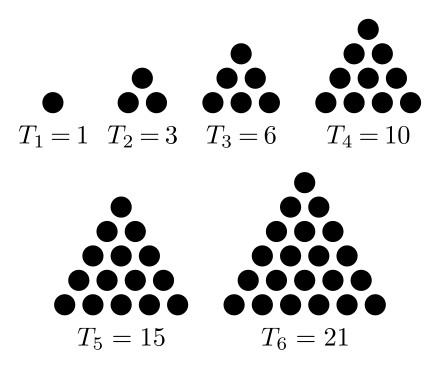
\includegraphics[frame,scale=0.45] {images/first_six_triangular_numbers.png}}
\caption{The First Six Triangular Numbers \cite{wiki:triangle_numbers}}
\label{fig:triangle_numbers}
\end{figure}


% \noindent
% Since $T_n$ is just the sum of the integers from 1 to $n$ we
% can easily calculate the first few values of $T_n$, which are 
% 1, 3, 6, 10, 15, 21, 28, 36, 45, 55, 66, 78, 91, 105 and so on
% (note that some authors include 0 in the triangular number
% sequence). 

\bigskip
\noindent
Ok, but what is the general form of $T_n$?  Since $T_n$ is the
sum of the first $n$ integers we know that\footnote{The great
mathematician Carl Friedrich Gauss is said to have discovered the
consecutive integer formula while still at primary school
\cite{gauss_on_arithmetic_sequences}.}

\medskip
\begin{equation}
T_{n} = \sum _{k=1}^{n} k=1+2+3+\dotsb +n = {\frac {n(n+1)}{2}} = {n+1 \choose 2}
\label{eqn:T_n}
\end{equation}

\bigskip
\noindent
As an aside, there is an interesting relationship between the
triangular numbers and Pascal's Triangle
\cite{wiki:pascals_triangle}: if you start at the second row
(counting from zero) and second column (again counting from zero)
of Pascal's Triangle the corresponding diagonal contains the
triangular numbers. This is shown in Figure
\ref{fig:pascals_triangle}. Figure
\ref{fig:pascals_triangle_with_binomial_coefficients} shows Pascal's
Triangle with binomial coefficients (the triangular numbers are
shown in {\color{blue}{blue}}).
%
%
%
\medskip
\bigskip
\begin{figure}[H]
\center{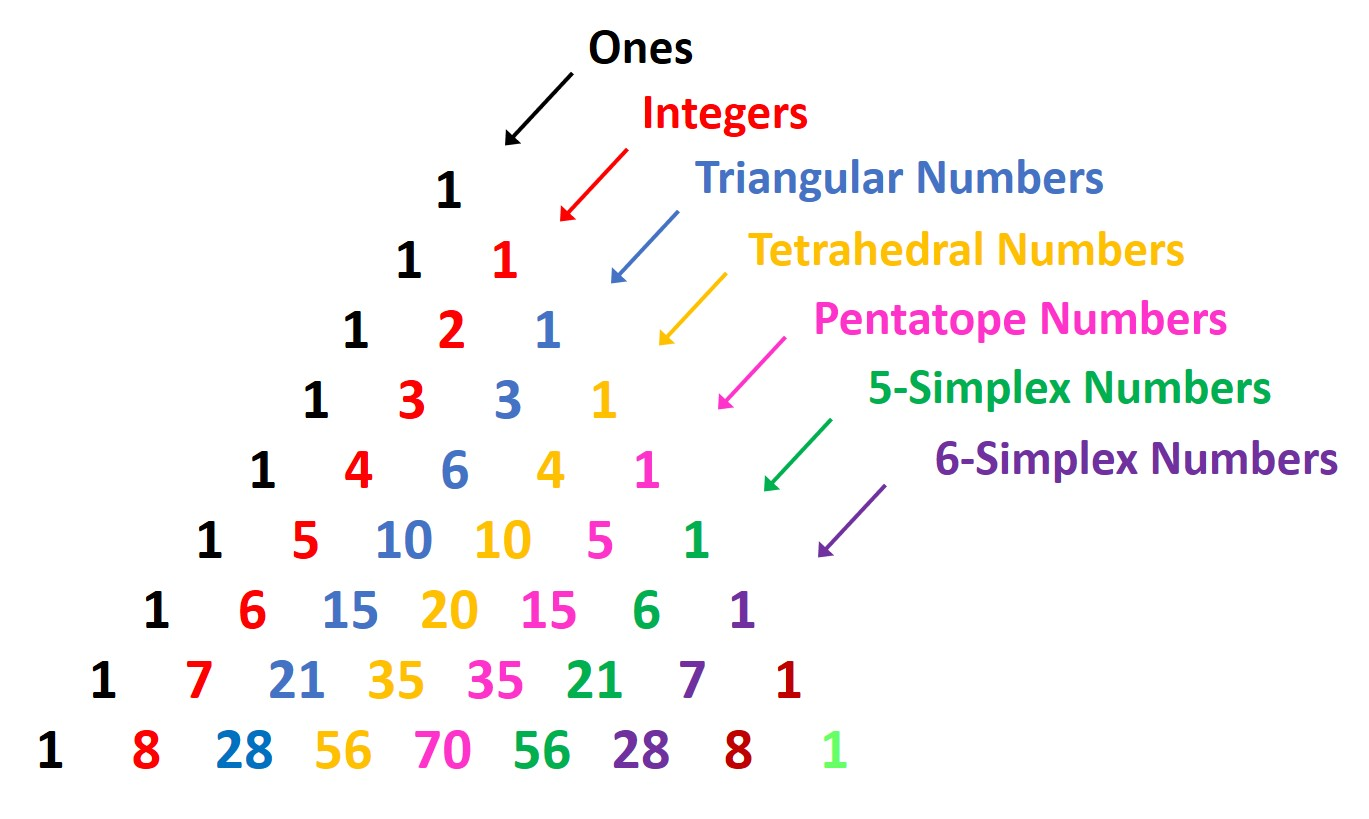
\includegraphics[frame,scale=0.45] {images/pascals_triangle.jpg}}
\caption{Number patterns in Pascal's Triangle \cite{mathaletes_corner_pascals_triangle}}
\label{fig:pascals_triangle}
\end{figure}
%
\newpage
%
%	Draw Pascal's Triangle with binomial coefficients. The triangular numbers
%	are shown in blue.
%
\newcommand \rows {8}                                                   % number of rows
%
%	Draw the picture
%
\begin{figure}[H]
\centering																% center everything
	\begin{tikzpicture} [framed,scale=0.90]								% put a frame on the tikzpicture 
		\foreach \n in {0,...,\rows} {                                  % iterate over rows
		  \foreach \k in {0,...,\n} {                                   % iterate over columns
		    \node at (\k-\n/2,-\n) {                                    % put the coefficient here
		      \ifnum \k = 2 {\color{blue} $\mathbf{\binom{\n}{\k}}$}    % k = 2 => triangular number
		      \else         {\color{black}$\mathbf{\binom{\n}{\k}}$}	% otherwise make it black
                      \fi};												% end \ifnum
		  }																% end \foreach \k ...
		}																% end \foreach \n ...
	\end{tikzpicture}													% end tikzpicture
\caption{Pascal's Triangle with Binomial Coefficients}
\label{fig:pascals_triangle_with_binomial_coefficients}
\end{figure}

\bigskip
\section{The Sum of the Reciprocals of the Triangular Numbers}
\label{sec:reciprocals}
All of this is good, but back to the question: what is the sum of
the reciprocals of the triangular numbers? 

\bigskip
\noindent
Well, first, the sum ${\displaystyle \sum\limits_{n=1}^{N} \frac{1}{T_n}}$ 
looks like


\begin{equation*}
\begin{array}{lllll}
{\displaystyle \sum \limits_{n=1}^{N} \frac{1}{T_n}}
&=& {\displaystyle  \sum _{n=1}^{N} \frac{1}{\frac{n(n+1)}{2}}}
                &\qquad \qquad \qquad \mathrel{\#} \text{definition of $T_n$ 
                (Equation (\ref{eqn:T_n}))} \\
[15pt]
&=& {\displaystyle \sum _{n=1}^{N} \frac{2}{n (n+1)}}
                &\qquad \qquad \qquad \mathrel{\#} \text{simplify} \\
[15pt]
&=& {\displaystyle  2 \sum _{n=1}^{N} \left (\frac{1}{n} \right)
\left ( \frac{1}{n+1} \right )}
                &\qquad \qquad \qquad \mathrel{\#} \text{pull 2 out of the sum 
                and group terms} \\
[15pt]
&=& {\displaystyle  2 \sum\limits_{n=1}^N \left( \frac{1}{n} -
\frac{1}{n+1} \right)}
                &\qquad \qquad \qquad \mathrel{\#} 
                \text{Equation (\ref{eqn:trick_1})}
\end{array}
\end{equation*}

\bigskip
{\setstretch{1.90} 
\noindent
We saw in Section \ref{sec:telescoping_series} that
${\displaystyle \lim_{N \to \infty} \sum\limits_{n=1}^N \left(
\frac{1}{n} - \frac{1}{n+1} \right ) = \lim_{N \to \infty} \left
[ 1 - \frac{1}{N+1} \right ] = 1}$ and we know from the above
that the infinite sum of the reciprocals of the triangular
numbers is twice this limit. So we know that \par}

\bigskip
\begin{equation*}
\sum \limits_{n=1}^{\infty} \frac{1}{T_n} = 2 \Bigg [  \lim_{N
\to \infty} \left  [ 1  - \frac{1}{N+1} \right ] \Bigg ]= 2 \cdot
1 =  2 
\end{equation*}


\section{Conclusions}
Equation (\ref{eqn:trick_1}) turns out to be very useful,
especially when evaluating infinite telescoping series. We also
saw in Section \ref{sec:reciprocals} that interestingly, the
infinite sum of the reciprocals of the triangular numbers equals
two, that is, 

\begin{equation*}
\displaystyle \sum \limits_{n=1}^{\infty} 
\frac{1}{T_n} =  2
\end{equation*}

\bigskip
\noindent
As we saw in Section \ref{sec:telescoping_series}, the evaluation
of this sum makes heavy use of a telescoping series described by
Equation (\ref{eqn:trick_1}).
%
%
%
\section*{Acknowledgements}
%
%	LaTeX source on overleaf.com
%
\section*{\LaTeX \hspace{0.10 mm} Source}
\url{https://www.overleaf.com/read/czsqywqhccfw}
%
%	get a bibliography
%
%	Note:.bib files go in ~/Library/texmf/bibtex/bib with TeXShop (MacTeX).
%	You can also use an absolute path, e.g. \bibliography{/Users/dmm/papers/bib/qc}
%
\bibliographystyle{plain}
\bibliography{qc}
%
%	done
%
\end{document} 

